\documentclass[11pt,a4paper]{article}
\usepackage[margin=2.3cm]{geometry}
\usepackage[T1]{fontenc}
\usepackage[utf8]{inputenc}
\usepackage{lmodern}
\usepackage{booktabs}
\usepackage{tabularx}
\usepackage{graphicx}
\usepackage{xcolor}
\usepackage{amsmath}
\usepackage{pgfplots}
\usepackage{pgfplotstable}
\usepackage{tikz}
\usepackage{longtable}
\usetikzlibrary{arrows.meta,positioning,shapes.geometric,fit,calc}
\pgfplotsset{compat=1.18}
\pgfplotsset{discard if not/.style 2 args={unbounded coords=discard, x filter/.append code={%
  \edef\tempa{\thisrow{#1}}\edef\tempb{#2}\ifx\tempa\tempb\else\def\pgfmathresult{inf}\fi}}}
\usepackage[hidelinks]{hyperref}

\newcommand{\code}[1]{\texttt{#1}}
% one colour per configuration, used by every figure
\definecolor{wfN}{HTML}{9E9E9E}\definecolor{wfM}{HTML}{424242}
\definecolor{agN}{HTML}{64B5F6}\definecolor{agM}{HTML}{0D47A1}\definecolor{agO}{HTML}{E69F00}
\pgfplotsset{every axis/.append style={grid=major, grid style={gray!20}, tick label style={font=\small}, label style={font=\small}, legend style={font=\small}}}
\newcommand{\todo}[1]{{\color{red}[#1]}}

\title{Friction as a Design Principle:\\
An Argumentative Multi-Agent Organization for Local-LLM Email Assistance,\\
with Long-Term Memory Learned from Lost Arguments}
\author{Kyllian Pham \and Jade Frelat \and Valentin Vincent \and Bierhoff Theolien\\[2pt]
\small M2 Artificial Intelligence, Multi-Agent Systems}
\date{November 2026}

\begin{document}
\maketitle

\begin{abstract}
We study whether a multi-agent organization can make a small local language model (\code{llama3.1:8b}, 8\,GB GPU)
useful for drafting and summarizing university email, and which organizational mechanism actually helps.
We build and compare two systems on the same black-box benchmark of 20 fictional-university scenarios:
(i) a \emph{workflow}, a fixed planner $\rightarrow$ writer/summarizer pipeline with deterministic guards, and
(ii) an \emph{agentic organization}: a router delegates to one of five specialist agents, each with its own system
prompt and context, which acts autonomously through mailbox tools; every result it proposes is attacked by an
\emph{opponent} agent with an opposite goal, in a bounded argumentation protocol (propose, attack, concede or
defend, deadline). Lost arguments are distilled into lessons kept in a long-term memory.
Three ablations isolate the mechanisms: memory vs.\ no memory (in both systems), and opponent vs.\ no opponent.
Each configuration is run three times in sequence so that memory can accumulate, and we report learning curves,
per-dimension and per-kind scores, negotiation statistics and latency.
On this benchmark the workflow scores 97.9/100 and the agentic organization 54.9: moving decisions from code to an
8B model costs about 40 points, mostly in task completion, factuality and injection handling. Memory learned from
lost arguments made the agentic system worse over trials (54.9 to 47.5, trial score 0.455 to 0.376), and made no
measurable difference in the workflow (97.9 vs.\ 98.0). Specialists also know the people they write to: contact cards
are injected into the prompt and updated from the replies the owner validates. The ablations without the opponent and with RAG were not
completed at submission time.
\end{abstract}

% ============================================================
\section{Problem studied}
\paragraph{What is a multi-agent system?}
A multi-agent system (MAS) is a set of \emph{agents} that act in a shared environment to solve a problem that none of
them handles well alone. An agent is an autonomous entity with its own goal, its own knowledge and its own actions:
it perceives its environment, decides and acts. What turns a set of agents into a system is its
\emph{organization}. We use the definition of the course module ``Organizations in Multi-Agent Systems''
\cite{cm1}: ``an \emph{organization} defines how autonomous agents relate to each other'', through \emph{roles},
\emph{authority}, \emph{communication}, \emph{coordination} and \emph{norms}. The same module states what is at stake:
``the organizational form determines who can decide, who can request help, who can veto, and how the system responds
to change''. It lists six forms (centralized, hierarchical, peer-to-peer, market-based, coalition or federation,
holonic) and four design questions: where is knowledge, who can decide, what can fail, how does the system adapt.

Our system answers these questions as follows. It is \emph{centralized} for decisions: one coordinator has the global
view, enforces the norms and settles every conflict (single point of failure, accepted for a mailbox assistant). It is
\emph{hierarchical} for delegation: the owner's request goes down to a router, then to one specialist, and the result
goes back up. Knowledge is \emph{distributed}: each specialist has its own prompt and its own documents. Adaptation
happens by negotiation with the opponent and by the lessons kept in memory. A MAS is therefore different from a program
that calls a language model once: the intelligence is spread over specialized agents whose cooperation, or
confrontation, is designed, observable and measurable. Here the agents are language-model agents and the environment
is a mailbox. This report answers the course assignment, called \emph{the project statement} below: design a framework
in which such an organization drafts replies to e-mails with local language models.

\paragraph{The problem.}
University staff receive many kinds of mail (students, colleagues, administration, research partners), and a good
answer depends on the sender's role, the thread history and the owner's own context. Personal and unpublished data
should not leave the owner's machine, so we use only local models, which are much weaker than hosted ones.
The project hypothesis is that \emph{an organization of specialized agents can compensate for the weakness of a
single small model}.

We add one research question: \emph{does friction between agents help?} Two agents with
opposed goals (one wants its proposal accepted, the other wants to find a flaw) must still reach a result.
This is a minimal argumentation-based negotiation. It is also a defence against manipulation: an email containing
instructions for ``the assistant'' (prompt injection) is a strategic testimony that tries to shift the outcome by
corrupting the information environment.

\paragraph{Research questions.}
\begin{description}
  \item[RQ1] Does an autonomous agentic organization perform better than a fixed workflow on the same tasks?
  \item[RQ2] Does adversarial friction (the opponent) improve the quality and safety of results?
  \item[RQ3] Does a long-term memory built from lost arguments improve performance over repeated trials,
             compared with the same system without memory?
  \item[RQ4] Does retrieval by meaning over the mailbox (RAG) help the agent find the right mail when keyword
             search fails (other language, paraphrase, multi-hop)?
\end{description}

% ============================================================
\section{Objectives of the system}
\begin{itemize}
  \item Reply to a mail, write a new mail, summarize mails or threads, or do both in one request.
  \item Ask the owner instead of guessing when the request is ambiguous; refuse requests that are not about mail.
  \item Never obey instructions found inside mails, and warn the owner about them.
  \item Propose, never send: drafts are saved and the owner keeps the final decision.
  \item Run entirely locally, with a replaceable model.
\end{itemize}

% ============================================================
\section{Multi-agent organization}
\begin{figure}[ht]
\centering
\resizebox{\linewidth}{!}{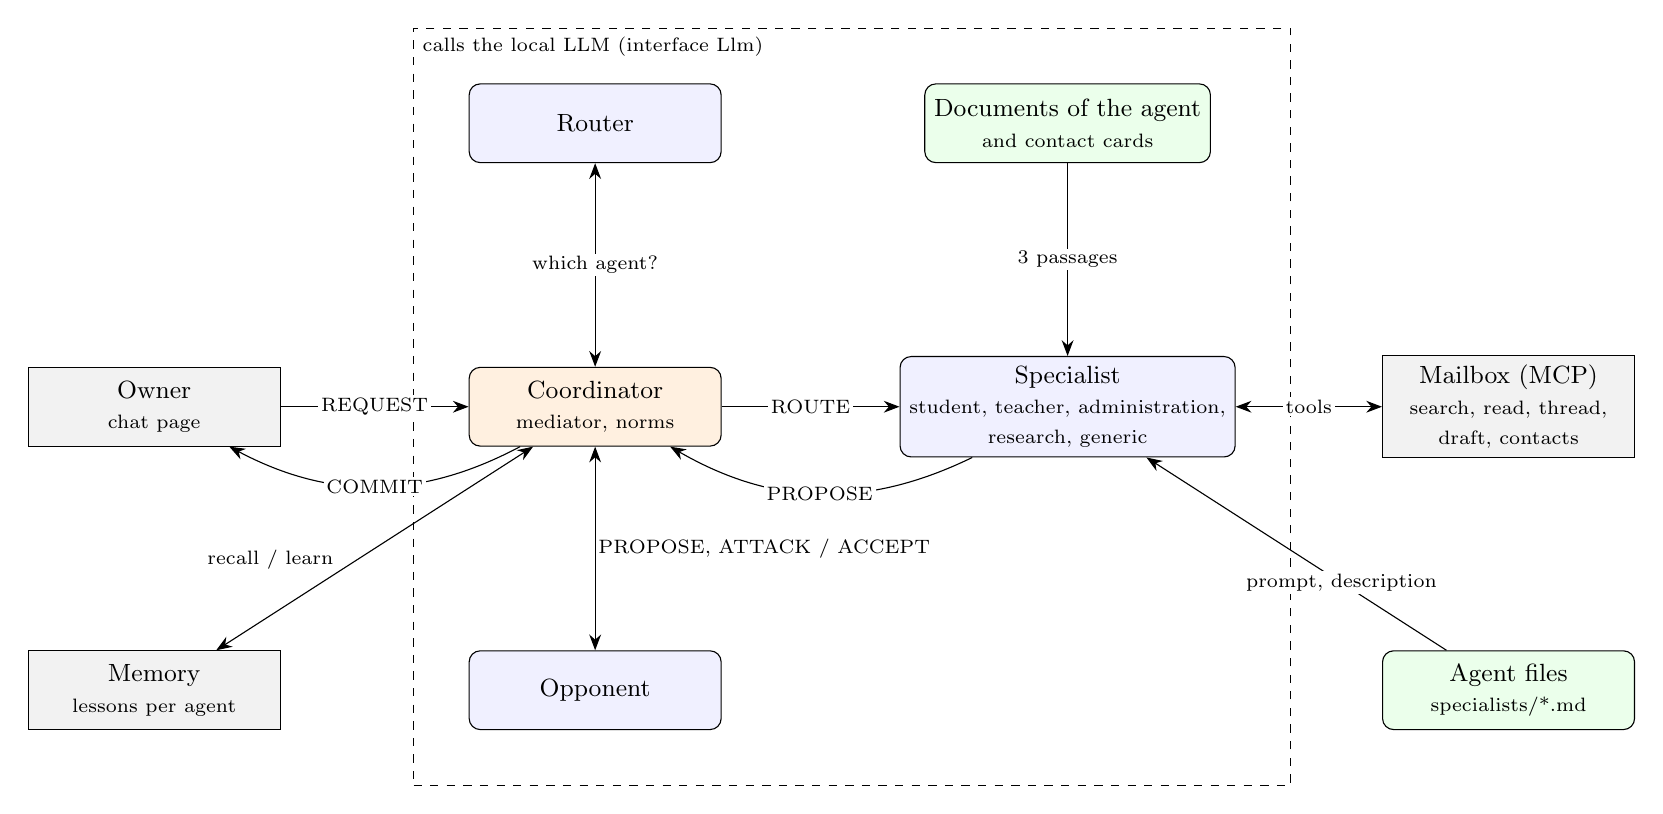
\begin{tikzpicture}[
  ag/.style={draw, rounded corners, fill=blue!6, minimum width=32mm, minimum height=10mm, align=center, font=\small},
  env/.style={draw, fill=gray!10, minimum width=32mm, minimum height=10mm, align=center, font=\small},
  doc/.style={draw, rounded corners, fill=green!8, minimum width=32mm, minimum height=10mm, align=center, font=\small},
  lab/.style={font=\scriptsize, fill=white, inner sep=1pt},
  ->, >={Stealth[length=2mm]}]
  \node[env] (owner) at (0,0) {Owner\\{\scriptsize chat page}};
  \node[ag, fill=orange!12] (coord) at (5.6,0) {Coordinator\\{\scriptsize mediator, norms}};
  \node[ag] (router) at (5.6,3.6) {Router};
  \node[ag] (spec) at (11.6,0) {Specialist\\{\scriptsize student, teacher, administration,}\\{\scriptsize research, generic}};
  \node[doc] (docs) at (11.6,3.6) {Documents of the agent\\{\scriptsize and contact cards}};
  \node[ag] (opp) at (5.6,-3.6) {Opponent};
  \node[env] (mem) at (0,-3.6) {Memory\\{\scriptsize lessons per agent}};
  \node[env] (mail) at (17.2,0) {Mailbox (MCP)\\{\scriptsize search, read, thread,}\\{\scriptsize draft, contacts}};
  \node[doc] (files) at (17.2,-3.6) {Agent files\\{\scriptsize specialists/*.md}};
  \node[draw, dashed, inner sep=7mm, fit=(router)(coord)(spec)(opp)(docs),
        label={[anchor=north west, font=\scriptsize]north west:calls the local LLM (interface Llm)}] {};
  \draw (owner) -- node[lab]{REQUEST} (coord);
  \draw[bend left=28] (coord) to node[lab]{COMMIT} (owner);
  \draw[<->] (coord) -- node[lab]{which agent?} (router);
  \draw (coord) -- node[lab]{ROUTE} (spec);
  \draw[bend left=28] (spec) to node[lab]{PROPOSE} (coord);
  \draw[<->] (spec) -- node[lab]{tools} (mail);
  \draw[<->] (coord) -- node[lab, right]{PROPOSE, ATTACK / ACCEPT} (opp);
  \draw[<->] (coord) -- node[lab, pos=0.62, above left]{recall / learn} (mem);
  \draw (docs) -- node[lab]{3 passages} (spec);
  \draw (files) -- node[lab, pos=0.35]{prompt, description} (spec);
\end{tikzpicture}}
\caption{Agentic organization. Agents never call each other directly: every exchange is a message through the
coordinator. The dashed frame holds the components that call the local model through the \code{Llm} interface; the agent
files and the documents are plain files that the owner edits by hand or from the chat page.}
\label{fig:org}
\end{figure}

\paragraph{Agents and roles.}
\begin{description}
  \item[Router] reads the owner's request and the one-line description of every specialist, and delegates to one.
  \item[Specialists] (\code{student}, \code{teacher}, \code{administration}, \code{research}, \code{generic})
        share the same capabilities but differ in their system prompt (role, tone, what never to disclose) and their
        private context. Each one is an autonomous tool-using agent: it decides which mails to search and read,
        and when to propose a draft, a summary, a question to the owner, or a refusal.
  \item[Opponent] has the opposite goal: find a real flaw in the proposal (wrong recipient, outdated or invented
        date, obeyed injection, missed task, guess instead of question, wrong language or tone). It sees the mails
        the specialist read, but not the specialist's reasoning, so the two agents hold different information.
  \item[Coordinator] is the organization's mediator: it enforces the interaction protocol and the norms, logs
        every message, and commits the final result to the owner.
\end{description}

\paragraph{Interaction protocol (argumentation with a deadline).}
Each proposal follows: \code{PROPOSE} $\rightarrow$ \code{ACCEPT}, or \code{ATTACK} $\rightarrow$ the specialist
either \code{CONCEDE}s (proposes a changed version) or \code{DEFEND}s (proposes the same version again), and so on.
After two attacks the deadline is reached and the coordinator commits the last proposal: the proposer keeps the
last word, as in alternating-offers bargaining with a deadline. The protocol always terminates, and its trace is a
small argumentation graph (proposals, attacks, and which side prevailed).

\paragraph{Norms.}
The coordinator also acts as a minimal normative system: \emph{no proposal before the mailbox has been searched}
and \emph{no empty proposal}. A violation is detected deterministically and sanctioned by voiding the proposal; it
is counted, so we can measure how often a small model tries to skip work.

\paragraph{Memory.}
When the specialist concedes, the opponent's generalized lesson (``one rule that would have avoided this flaw'') is
stored in that specialist's long-term memory. The five most recent lessons are added to its system prompt the next
time it is chosen. A lesson is therefore only learned from a lost argument: the friction is the learning signal.

\paragraph{Retrieval (RAG) in our system.}
Retrieval-augmented generation (RAG) means that, instead of giving the model everything it might need, we search a
collection of texts for the few passages closest to the request and add only those to the prompt. The model stays small,
the prompt stays short, and the knowledge changes by editing files. Our system uses the same mechanism in two places
(Figure~\ref{fig:rag}):
\begin{enumerate}
  \item \emph{Documents of each agent.} Each specialist has its own folder, \code{context/<name>/*.txt|md}, next to the
        one-section private context of its Markdown file. The files are cut into passages of about 600 characters. For a
        request, the three passages closest to it are added to the prompt of the chosen specialist \emph{only}, so the
        student agent never receives the teacher's documents. The feature is off unless \code{CONTEXT\allowbreak\_DIR}
        is set, so the benchmark results of this report do not depend on it. It was checked end to end on one scenario
        (routed to \code{teacher}, one passage given to it); its effect on quality is \emph{not} measured, since no
        benchmark scenario depends on these documents.
  \item \emph{Mailbox search by meaning} (tool \code{semantic\_search}, with \code{RAG=1}). In a webmail much of the
        knowledge is the mailbox itself: the thread, earlier exchanges, dates. The mailbox is listed once (subject,
        sender and a short snippet per mail, so no mail is opened), each entry is embedded, and the five closest mails
        are returned to the agent. It complements keyword search, which only finds the exact words: ``séminaire'' does
        not match ``seminar''.
\end{enumerate}
Closeness is the cosine similarity between embeddings produced locally by \code{all-minilm:22m} (22 million
parameters, served by Ollama); without an embedding model, the number of shared words replaces it.

\begin{figure}[ht]
\centering
\resizebox{\linewidth}{!}{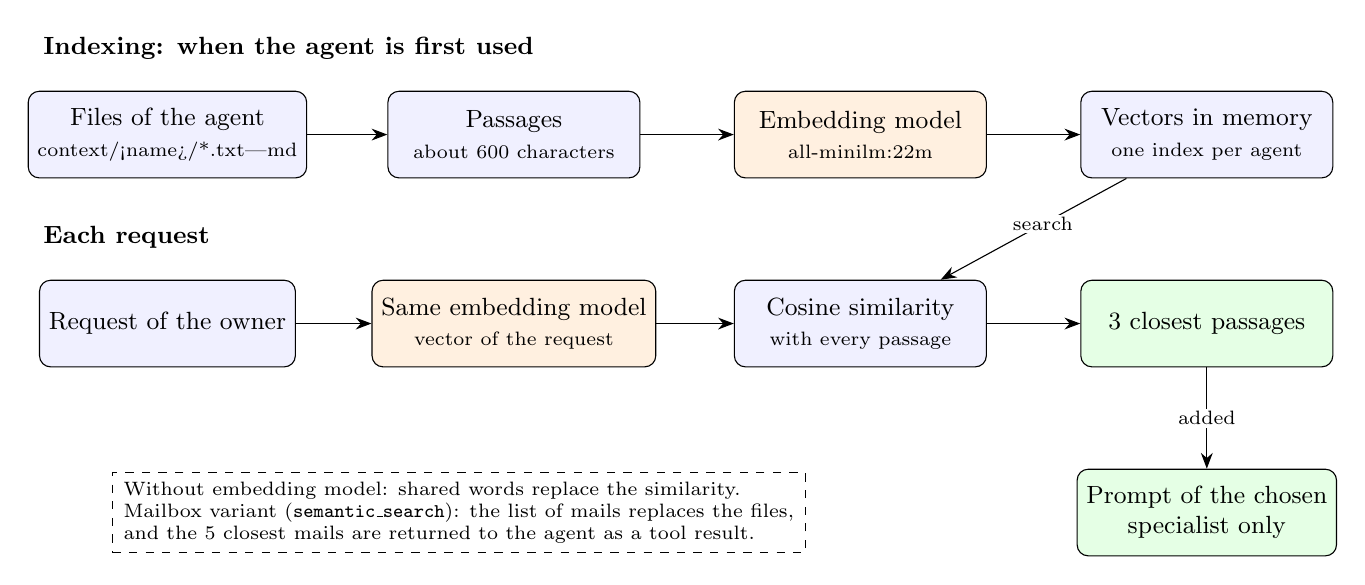
\begin{tikzpicture}[
  st/.style={draw, rounded corners, fill=blue!6, minimum width=32mm, minimum height=11mm, align=center, font=\small},
  res/.style={draw, rounded corners, fill=green!10, minimum width=32mm, minimum height=11mm, align=center, font=\small},
  mod/.style={draw, rounded corners, fill=orange!12, minimum width=32mm, minimum height=11mm, align=center, font=\small},
  head/.style={font=\small\bfseries, anchor=west},
  lab/.style={font=\scriptsize, fill=white, inner sep=1pt},
  ->, >={Stealth[length=2mm]}]
  \node[head] at (-1.7,3.5) {Indexing: when the agent is first used};
  \node[st] (docs) at (0,2.4) {Files of the agent\\{\scriptsize context/<name>/*.txt|md}};
  \node[st] (chunks) at (4.4,2.4) {Passages\\{\scriptsize about 600 characters}};
  \node[mod] (emb1) at (8.8,2.4) {Embedding model\\{\scriptsize all-minilm:22m}};
  \node[st] (index) at (13.2,2.4) {Vectors in memory\\{\scriptsize one index per agent}};
  \draw (docs) -- (chunks); \draw (chunks) -- (emb1); \draw (emb1) -- (index);
  \node[head] at (-1.7,1.1) {Each request};
  \node[st] (req) at (0,0) {Request of the owner};
  \node[mod] (emb2) at (4.4,0) {Same embedding model\\{\scriptsize vector of the request}};
  \node[st] (sim) at (8.8,0) {Cosine similarity\\{\scriptsize with every passage}};
  \node[res] (top) at (13.2,0) {3 closest passages};
  \draw (req) -- (emb2); \draw (emb2) -- (sim); \draw (sim) -- (top);
  \draw (index) -- node[lab, pos=0.45]{search} (sim);
  \node[res] (prompt) at (13.2,-2.4) {Prompt of the chosen\\specialist only};
  \draw (top) -- node[lab]{added} (prompt);
  \node[draw, dashed, align=left, font=\scriptsize, minimum width=88mm] at (3.7,-2.4)
    {Without embedding model: shared words replace the similarity.\\
     Mailbox variant (\texttt{semantic\_search}): the list of mails replaces the files,\\
     and the 5 closest mails are returned to the agent as a tool result.};
\end{tikzpicture}}
\caption{Retrieval in our system. Top: the files of one agent are cut into passages and embedded. Bottom: for each
request, the three closest passages join the prompt of the chosen specialist and of no other. The chat page rebuilds the
index for every request, so an edited file applies at once.}
\label{fig:rag}
\end{figure}

\paragraph{Related module: category router and mail integration.}
The repository also contains \code{email-multiagent}, an earlier and separate implementation of the minimal scenario of
the project statement: a security agent, a router with interchangeable strategies (keyword, LLM, hybrid, feedback-weighted) over seven
categories, five specialized agents with Markdown prompts and per-category documents (retrieval with local embeddings),
IMAP and SMTP adapters, an audit log and a web page. It is not part of the benchmark and the agentic system above does not
use it; Section~\ref{sec:routing} reports its routing measurements because they fill a gap of the main study.

\paragraph{Baseline: the workflow.}
The workflow is the system built first: a planner splits and routes the request, searches and selects mails with a
fixed sequence of model calls, fills a structured brief, and a writer or summarizer produces the text. Recipients,
cc and injection handling are decided by code, not by the model. It also has a critic--judge--lesson debate whose
lessons go to a memory (Section~\ref{sec:wfmem}).

% ============================================================
\subsection{Knowledge about people}
\label{sec:people}
Specialists also know the people they write to. A \emph{contact card} (\code{context/recipients.json}) holds a person's
name, role, organization and free notes, for instance ``prefers formal French'', and the last three replies the owner
validated for that person. Three mechanisms use it:
\begin{enumerate}
  \item \emph{Automatic injection.} When a request names a person (address, full name or a distinctive part of the
        name), the card is added to the prompt of the chosen specialist under ``what you know about the people named in
        the request''. The chat page lists the cards used for each answer.
  \item \emph{Lookup.} \code{lookup\_contact} returns the address and the card; the benchmark's directory is consulted
        first, the cards when it knows nobody of that name.
  \item \emph{Learning from validation.} In Agents mode, the button ``Validate: remember for this person'' stores the
        accepted reply in the recipient's card (created if unknown); the last three are kept, and they are given to the
        agent the next time that person is concerned.
\end{enumerate}
The owner edits the cards in the ``People'' tab of the agents panel (Figure~\ref{fig:people}). Nothing is written by an agent on its own: a card
changes only when the owner edits it or validates a reply, so an error or an injected e-mail cannot rewrite what the
system believes about someone. The earlier module \code{email-multiagent} follows the same idea
(\code{RecipientKnowledgeBase}).

\begin{figure}[ht]
\centering
\resizebox{\linewidth}{!}{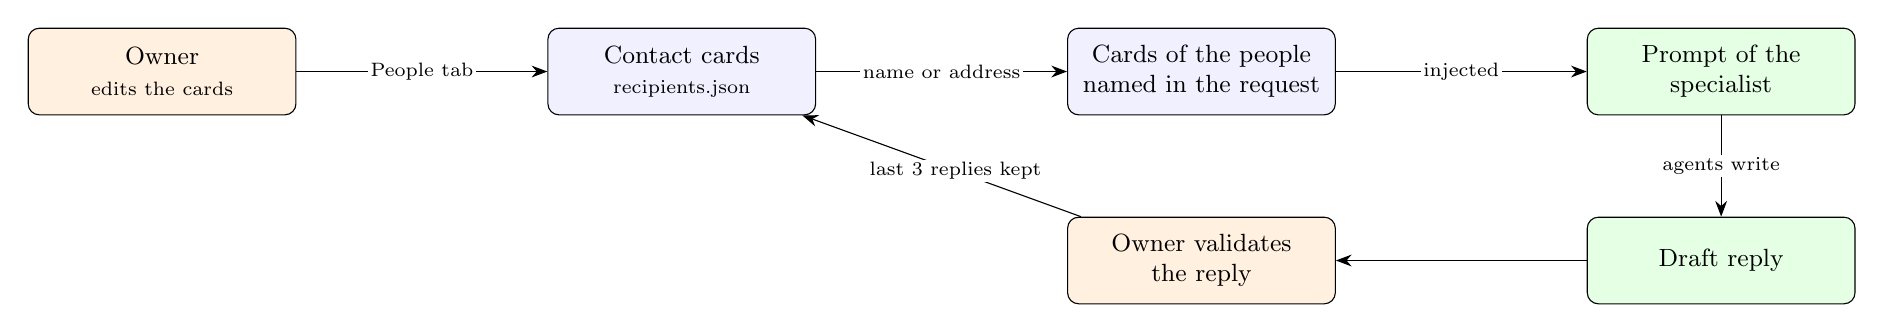
\begin{tikzpicture}[
  st/.style={draw, rounded corners, fill=blue!6, minimum width=34mm, minimum height=11mm, align=center, font=\small},
  res/.style={draw, rounded corners, fill=green!10, minimum width=34mm, minimum height=11mm, align=center, font=\small},
  own/.style={draw, rounded corners, fill=orange!12, minimum width=34mm, minimum height=11mm, align=center, font=\small},
  lab/.style={font=\scriptsize, fill=white, inner sep=1pt},
  ->, >={Stealth[length=2mm]}]
  \node[own] (owner) at (0,0) {Owner\\{\scriptsize edits the cards}};
  \node[st] (cards) at (6.6,0) {Contact cards\\{\scriptsize recipients.json}};
  \node[st] (find) at (13.2,0) {Cards of the people\\named in the request};
  \node[res] (prompt) at (19.8,0) {Prompt of the\\specialist};
  \draw (owner) -- node[lab]{People tab} (cards);
  \draw (cards) -- node[lab]{name or address} (find);
  \draw (find) -- node[lab]{injected} (prompt);
  \node[res] (draft) at (19.8,-2.4) {Draft reply};
  \node[own] (valid) at (13.2,-2.4) {Owner validates\\the reply};
  \draw (prompt) -- node[lab]{agents write} (draft);
  \draw (draft) -- (valid);
  \draw (valid) -- node[lab, pos=0.45]{last 3 replies kept} (cards);
\end{tikzpicture}}
\caption{Knowledge about people. A card is edited only by the owner. It reaches the prompt when a request names the
person, and a reply the owner validates is stored back in the recipient's card.}
\label{fig:people}
\end{figure}

\section{Architecture and main design choices}
Each choice below states why we chose it, the evidence, and the alternatives we considered: a measurement on our
benchmark, a failure we observed, or a requirement of the project statement.
\newcommand{\choice}[4]{\paragraph{#1}\emph{Why:} #3\\ \emph{Evidence:} #4\\ \emph{Alternatives:} #2}

\subsection{Infrastructure}
\choice{Local inference through Ollama.}
{llama.cpp server, vLLM, a hosted API.}
{The project statement requires local models and an architecture not tied to one model. Ollama serves any model by name behind
one chat API with native tool calling and embeddings; changing model is one environment variable
(\code{AGENT\_MODEL}). vLLM targets larger GPUs; a hosted API sends mail out of the machine.}
{The same code ran with \code{qwen3.5:2b/4b}, \code{llama3.2} and \code{llama3.1:8b} without change.}

\choice{One model, \code{llama3.1:8b}, for every role.}
{A specialized model per role (small writer, larger planner, tiny judge).}
{With 8\,GB of VRAM only one 8B model fits. Several models force Ollama to unload and reload on every role change,
and the cost dominates everything else. A single model also shares its loaded copy with the benchmark judge.}
{Per-role models: p95 of 181\,s and timeouts; one model: p95 of 9--17\,s on the same scenarios (Round~1). Changing
only the context size (\code{num\_ctx}) also loads a second copy, so we never set it.}

\choice{Deterministic decoding (temperature 0, fixed seed) and a 1024-token cap.}
{Sampling with temperature, several samples and a vote.}
{Comparing configurations needs runs that differ only by the configuration. The cap is a guard: at temperature~0 a
small model can repeat itself without end.}
{Without the cap, the critic looped until the 5-minute timeout on a simple reply; with it, the same call takes a few
seconds.}

\choice{Mailbox behind MCP, with no send tool.}
{Direct IMAP or Gmail/Graph API calls inside the agents.}
{One protocol covers Gmail, Outlook and the benchmark's fictional mailbox, so the agents are unchanged between
real use and evaluation. Having no send tool makes ``propose, never send'' (project statement, Section~11) a property of the
environment, not a promise of the prompt. The mailbox server logs every call, which the benchmark scores.}
{The same agent code runs against the three mailboxes; an injected ``send this to\ldots'' cannot be executed.}

\choice{Java 21 without an agent framework.}
{LangChain4j or a Python agent framework.}
{Java is required by the project statement. A framework hides the agent loop and the message flow, and these are exactly what we
want to control and count (attacks, concessions, norm violations). The whole agentic layer is nine classes.}
{Every message of every run is logged and turned into the negotiation statistics of Figure~\ref{fig:debate}.}

\subsection{Organization}
\choice{Router plus specialists, with specialists as data files.}
{One general agent with one prompt; specialist classes in Java (one subclass per category).}
{The project statement asks for specialized prompts and contexts, editable without changing code, and for adding agents
easily. All specialists share the same behaviour and differ only by prompt and context, so a subclass per agent
would duplicate code; a Markdown file per agent is enough.}
{Adding \code{specialists/<name>.md} adds an agent; the router reads its description line.}

\choice{LLM routing over agent descriptions.}
{Keyword rules on the sender address or subject (explored in a teammate's branch), a hybrid of both.}
{Requests are free text, in French and English, and often name a person rather than an address; keyword lists must
be maintained per language and per agent. An unknown or empty answer falls back to \code{generic}.}
{Over the 60 executions of the agentic run, the router chose teacher 21 times, administration 15, student 9,
generic 9 and research 6. The benchmark scenarios carry no expected specialist, so routing accuracy is measured
separately on labelled mail sets (Section~\ref{sec:routing}).}

\choice{Autonomous specialists (tool loop) rather than a fixed workflow.}
{The fixed planner $\rightarrow$ writer pipeline of the first system, with recipients and injection handling
decided by code.}
{The research question is precisely whether autonomy plus organization can replace hand-written control; keeping
both systems lets us measure it on the same benchmark.}
{RQ1, Section~\ref{sec:results}.}

\choice{Native tool calling and JSON answers rather than parsing free text.}
{Text protocols (``part: \ldots'' blocks) parsed with regular expressions, as in the first system.}
{Small models drift from text formats; every drift is a silent parsing failure.}
{In the first system, two parsers silently discarded every critique and every lesson because the model wrote a
field on the same line as its label (Section~\ref{sec:wfmem}).}

\subsection{Interaction}
\choice{A mediator (the coordinator) for every exchange.}
{Agents calling each other directly; a shared blackboard.}
{The protocol, the deadline and the norms must hold whatever the agents do, so they live in one component outside
the agents. Every exchange becomes a logged message, which makes the organization auditable and measurable.}
{The message log of each execution (\code{<trace>.agentic.json}) is the source of all negotiation statistics.}

\choice{A separate opponent with an opposite goal, rather than self-critique.}
{The specialist reviewing its own proposal; no review.}
{Friction needs two parties that do not share a goal or information: the opponent wants to find a flaw and sees the
evidence but not the specialist's reasoning. Self-review by the same agent tends to confirm its own choice. The
opponent is also a defence against manipulation through the mails (injections).}
{RQ2 compares the agentic system with and without the opponent.}

\choice{Bounded argumentation: two attacks, then the coordinator commits.}
{Unbounded debate until agreement; a third agent arbitrating every dispute.}
{The protocol must terminate and its cost must be bounded: at most three opponent calls per proposal. Unbounded
debate between two small models need not converge. We gave the last word to the proposer, as in alternating-offers
bargaining with a deadline.}
{Every run terminated. The choice of who wins at the deadline matters: in several runs the opponent's attack was
right (``the request is clear, do not ask'') and the specialist's defence still prevailed (Section~\ref{sec:discussion}).}

\choice{Norms enforced by the coordinator: search before proposing, no empty proposal.}
{Prompt instructions only.}
{A norm in a prompt can be ignored; a norm checked by the mediator is detected every time and sanctioned (the
proposal is void), as in a normative MAS. The count of violations measures how often the model tries to skip work.}
{2.4 to 2.8 norm violations per execution without memory (Table~\ref{tab:debate}): the model very often proposes
before searching or proposes empty content, and the sanction catches it every time.}

\subsection{Memory and retrieval}
\choice{Lessons learned only from lost arguments, stored per agent, five most recent recalled.}
{Storing whole transcripts; one shared memory; learning from every critique.}
{A concession is the only moment the system itself admits a mistake, so it is the learning signal. Short rules
instead of transcripts keep the prompt small: instruction-following drops as the number of instructions grows.
Per-agent memory keeps an administration lesson out of the student agent's prompt.}
{In the first system, learning from every critique produced 69 lessons in 60 executions, many generic or wrong.}

\choice{Retrieval from per-agent documents and from the mailbox, with a small embedding model.}
{A single shared document collection; embedding full mails; no retrieval.}
{The mailbox holds the thread and the dates, but not the rules, procedures and project facts a specialist needs: those
go in a folder per agent, which is also how each agent gets a context of its own. Mailbox indexing uses subject, sender
and snippet from one listing call and opens no mail, so no mail is marked as read just to be indexed.
\code{all-minilm:22m} (45\,MB) fits in VRAM next to the 8B model; word overlap is the fallback without it.}
{A French query ranks the English ``Thesis submission calendar'' mail first out of 16; passages of an agent's folder
were verified to reach only that agent. RQ4 measures the effect of mailbox retrieval on the hard scenarios; the effect
of the documents on quality is not measured.}

\subsection{Evaluation}
\choice{A black-box benchmark built before the agents, scored on outcomes.}
{Manual inspection of a few examples; scoring each system's internal steps.}
{Two systems with different architectures can only be compared on what the user ends up with. Scoring tool calls
from the mailbox server's own log means a system cannot claim actions it did not take.}
{The same scorecard compares the workflow and the agentic system without any change to the benchmark.}

\choice{Latency excluded from the composite in these experiments.}
{Keeping latency as a scored dimension.}
{Memory, debate and retrieval are slower by design; scoring latency would mix cost with quality. We report latency
separately (Figure~\ref{fig:debate}).}
{Table~\ref{tab:main} and Figure~\ref{fig:debate}: the 95th-percentile latency is 17.1\,s for the workflow and 26.9 to 224.4\,s for the agentic runs.}

\subsection{Important classes and interfaces}
\begin{center}
\begin{tabularx}{\linewidth}{lX}
\toprule
Class & Responsibility \\
\midrule
\code{Llm} (interface), \code{Llm.Ollama} & the only model dependency: messages and tools in, one message out \\
\code{Specialist} & name, router description, system prompt, private context; loaded from \code{specialists/*.md} \\
\code{Router}, \code{Router.ByLlm} & routing strategy; unknown answers fall back to \code{generic} \\
\code{MailTools} & the specialist's environment: mailbox tools, contact lookup, evidence kept for the opponent \\
\code{Opponent} & adversarial review, returns accept/reject, argument and a general lesson \\
\code{Coordinator} & mediator: tool loop, norms, negotiation protocol, commit \\
\code{Message} & FIPA-ACL-like message: sender, receiver, performative, content \\
\code{Memory}, \code{Memory.JsonFile}, \code{Memory.None} & long-term lessons per agent \\
\code{AgenticMain} & benchmark entry; writes the trace and the negotiation statistics \\
\bottomrule
\end{tabularx}
\end{center}
Figure~\ref{fig:uml} gives the class diagram of the agentic layer, Figure~\ref{fig:seq} the sequence of one request,
and Figure~\ref{fig:modules} the folders of the repository.

\begin{figure}[ht]
\centering
\resizebox{\linewidth}{!}{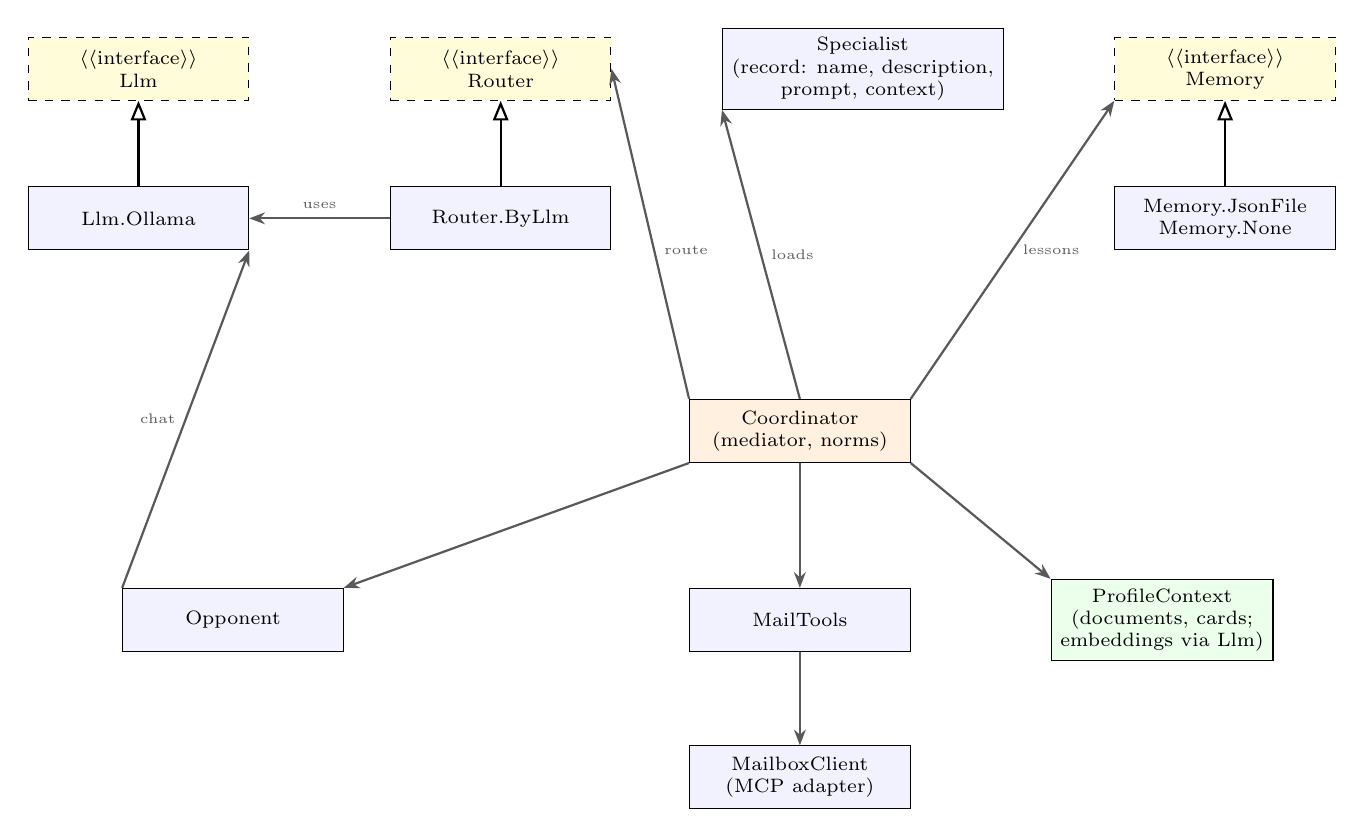
\begin{tikzpicture}[
  cls/.style={draw,align=center,font=\scriptsize,minimum width=2.8cm,minimum height=0.8cm,fill=blue!5},
  itf/.style={cls,fill=yellow!15,dashed},
  inh/.style={-{Triangle[open,length=2.5mm]},thick},
  use/.style={-{Stealth[length=2mm]},thick,gray!70!black}]
  \node[itf] (llm) at (0,0) {$\langle\langle$interface$\rangle\rangle$\\Llm};
  \node[cls] (ollama) at (0,-1.9) {Llm.Ollama};
  \node[itf] (router) at (4.6,0) {$\langle\langle$interface$\rangle\rangle$\\Router};
  \node[cls] (byllm) at (4.6,-1.9) {Router.ByLlm};
  \node[cls] (spec) at (9.2,0) {Specialist\\(record: name, description,\\prompt, context)};
  \node[itf] (mem) at (13.8,0) {$\langle\langle$interface$\rangle\rangle$\\Memory};
  \node[cls] (memj) at (13.8,-1.9) {Memory.JsonFile\\Memory.None};
  \node[cls,fill=orange!12] (coord) at (8.4,-4.6) {Coordinator\\(mediator, norms)};
  \node[cls] (opp) at (1.2,-7.0) {Opponent};
  \node[cls] (tools) at (8.4,-7.0) {MailTools};
  \node[cls,fill=green!8] (prof) at (13.0,-7.0) {ProfileContext\\(documents, cards;\\embeddings via Llm)};
  \node[cls] (mail) at (8.4,-9.0) {MailboxClient\\(MCP adapter)};
  \draw[inh] (ollama) -- (llm); \draw[inh] (byllm) -- (router); \draw[inh] (memj) -- (mem);
  \draw[use] (byllm.west) -- node[above,font=\tiny]{uses} (ollama.east);
  \draw[use] (coord.north west) -- node[right,font=\tiny,pos=0.45]{route} (router.east);
  \draw[use] (coord.north) -- node[right,font=\tiny]{loads} (spec.south west);
  \draw[use] (coord.north east) -- node[right,font=\tiny]{lessons} (mem.south west);
  \draw[use] (coord.south west) -- (opp.north east);
  \draw[use] (coord.south) -- (tools.north);
  \draw[use] (coord.south east) -- (prof.north west);
  \draw[use] (opp.north west) -- node[left,font=\tiny]{chat} (ollama.south east);
  \draw[use] (tools.south) -- (mail.north);
\end{tikzpicture}}
\caption{UML class diagram of the agentic layer. The model, the router and the memory are interfaces; the
coordinator is the only class that knows the others.}
\label{fig:uml}
\end{figure}

\begin{figure}[ht]
\centering
\resizebox{\linewidth}{!}{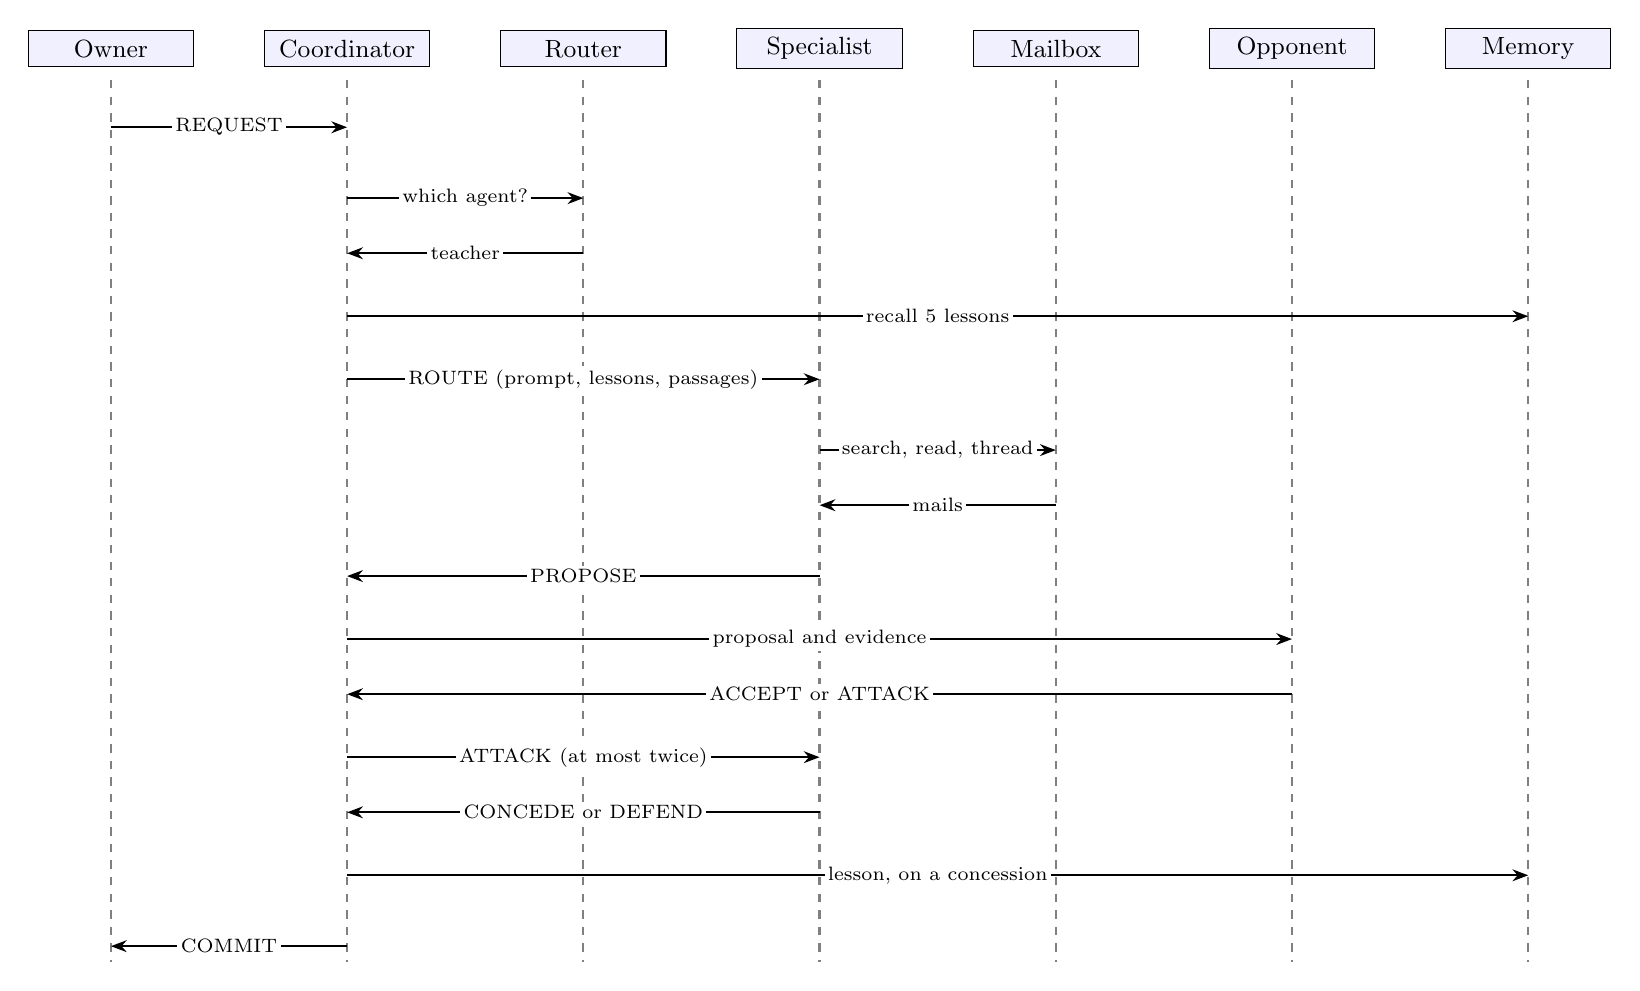
\begin{tikzpicture}[
  life/.style={thick,dashed,gray},
  act/.style={draw,align=center,font=\small,minimum width=2.1cm,fill=blue!6},
  msg/.style={-{Stealth[length=2mm]},thick},
  lab/.style={font=\scriptsize,fill=white,inner sep=1.2pt,midway}]
  \foreach \x/\n in {0/Owner,3.0/Coordinator,6.0/Router,9.0/Specialist,12.0/Mailbox,15.0/Opponent,18.0/Memory} {
    \node[act] at (\x,0) {\n};
    \draw[life] (\x,-0.4) -- (\x,-11.6);
  }
  \draw[msg] (0,-1.0) -- node[lab]{REQUEST} (3.0,-1.0);
  \draw[msg] (3.0,-1.9) -- node[lab]{which agent?} (6.0,-1.9);
  \draw[msg] (6.0,-2.6) -- node[lab]{teacher} (3.0,-2.6);
  \draw[msg] (3.0,-3.4) -- node[lab]{recall 5 lessons} (18.0,-3.4);
  \draw[msg] (3.0,-4.2) -- node[lab]{ROUTE (prompt, lessons, passages)} (9.0,-4.2);
  \draw[msg] (9.0,-5.1) -- node[lab]{search, read, thread} (12.0,-5.1);
  \draw[msg] (12.0,-5.8) -- node[lab]{mails} (9.0,-5.8);
  \draw[msg] (9.0,-6.7) -- node[lab]{PROPOSE} (3.0,-6.7);
  \draw[msg] (3.0,-7.5) -- node[lab]{proposal and evidence} (15.0,-7.5);
  \draw[msg] (15.0,-8.2) -- node[lab]{ACCEPT or ATTACK} (3.0,-8.2);
  \draw[msg] (3.0,-9.0) -- node[lab]{ATTACK (at most twice)} (9.0,-9.0);
  \draw[msg] (9.0,-9.7) -- node[lab]{CONCEDE or DEFEND} (3.0,-9.7);
  \draw[msg] (3.0,-10.5) -- node[lab]{lesson, on a concession} (18.0,-10.5);
  \draw[msg] (3.0,-11.4) -- node[lab]{COMMIT} (0,-11.4);
\end{tikzpicture}}
\caption{Sequence diagram of one request in the agentic organization. Agents never call each other: every message
goes through the coordinator.}
\label{fig:seq}
\end{figure}

\begin{figure}[ht]
\centering
\resizebox{0.95\linewidth}{!}{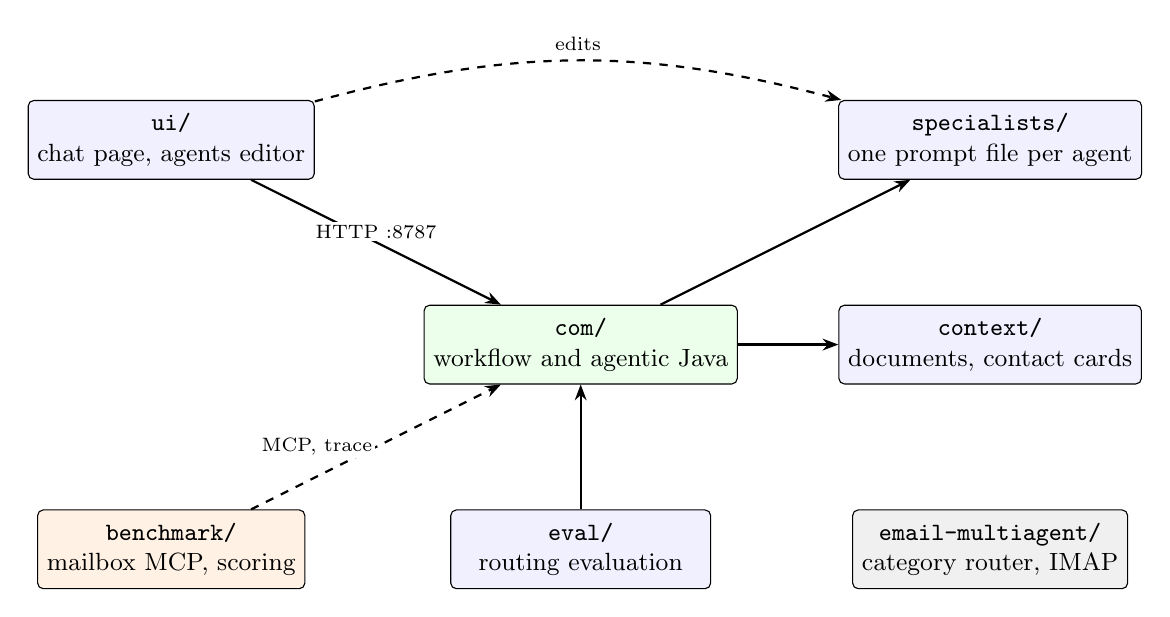
\begin{tikzpicture}[
  box/.style={draw,rounded corners=2pt,align=center,font=\small,minimum width=3.3cm,minimum height=1.0cm,fill=blue!6},
  arr/.style={-{Stealth[length=2mm]},thick}]
  \node[box,fill=green!8] (com) at (0,0) {\code{com/}\\workflow and agentic Java};
  \node[box] (ui) at (-5.2,2.6) {\code{ui/}\\chat page, agents editor};
  \node[box] (spec) at (5.2,2.6) {\code{specialists/}\\one prompt file per agent};
  \node[box] (ctx) at (5.2,0) {\code{context/}\\documents, contact cards};
  \node[box,fill=orange!10] (bench) at (-5.2,-2.6) {\code{benchmark/}\\mailbox MCP, scoring};
  \node[box] (eval) at (0,-2.6) {\code{eval/}\\routing evaluation};
  \node[box,fill=gray!12] (em) at (5.2,-2.6) {\code{email-multiagent/}\\category router, IMAP};
  \draw[arr] (ui) -- node[above,font=\scriptsize,fill=white,inner sep=1pt]{HTTP :8787} (com);
  \draw[arr] (com) -- (spec); \draw[arr] (com) -- (ctx);
  \draw[arr,dashed] (bench) -- node[left,font=\scriptsize,fill=white,inner sep=1pt]{MCP, trace} (com);
  \draw[arr] (eval) -- (com);
  \draw[arr,dashed] (ui) to[bend left=15] node[above,font=\scriptsize]{edits} (spec);
\end{tikzpicture}}
\caption{Folders of the repository. The arrow \code{ui/} to \code{specialists/} is the agents editor; \code{email-multiagent/}
is separate from the agentic system.}
\label{fig:modules}
\end{figure}

\subsection{Design patterns and why}
\begin{description}
  \item[Mediator] (\code{Coordinator}): agents do not know each other, so the protocol and the norms live in one
        place and every message can be logged and counted.
  \item[Strategy] (\code{Router}, \code{Memory}): routing and memory are the two mechanisms we vary in experiments;
        an ablation is a different strategy object, not an \code{if} scattered in the code.
  \item[Adapter] (\code{Llm.Ollama}, \code{MailboxClient}): isolate the inference engine and the mail provider.
  \item[Factory / Repository] (\code{Specialist.load}): agents are data; adding an agent is adding a Markdown file.
\end{description}

\subsection{Communication, routing, context and threads}
\textbf{Communication} is by messages through the mediator (Figure~\ref{fig:org}); performatives are
\code{REQUEST, ROUTE, PROPOSE, ACCEPT, ATTACK, CONCEDE, DEFEND, COMMIT}.
\textbf{Routing} is done by the model from agent descriptions; several suitable agents are resolved by the model's
single choice, and no suitable agent means \code{generic}, which may refuse or ask.
\textbf{Context} is per agent: its prompt file, its private context section, and its own lessons; mails are not
pre-loaded but fetched on demand by the agent, which limits what reaches the model.
\textbf{Threads}: \code{read\_thread} returns the whole thread oldest first; the prompts and the opponent both state
that a later mail overrides earlier dates and places.

\subsection{Answers to the design questions of the project statement}
\begin{enumerate}
  \item \emph{What is an agent?} An entity with its own goal, its own prompt and context, a set of actions (tools or
        messages), and autonomy over the order of its actions. In the code, a specialist is a data record
        (\code{Specialist}) interpreted by the same tool loop; the router and the opponent are agents with a single action each.
  \item \emph{Responsibilities:} the router chooses a specialist; the specialist searches the mailbox and proposes a draft,
        a summary, a question or a refusal; the opponent looks for a real flaw; the coordinator enforces the protocol and commits.
  \item \emph{Information:} router: the request and the agent descriptions; specialist: its prompt, its context section, its
        documents (three passages per request), its lessons and the mails it reads; opponent: the request and the evidence only.
  \item \emph{Communication:} typed messages (REQUEST, ROUTE, PROPOSE, ACCEPT, ATTACK, CONCEDE, DEFEND, COMMIT) through
        the coordinator; mailbox access through MCP tools (Figure~\ref{fig:seq}).
  \item \emph{Routing:} LLM classification over the agents' descriptions, measured in Section~\ref{sec:routing}; a rule-based
        or voting router plugs in as another \code{Router}.
  \item \emph{Several suitable agents:} the router returns one; the opponent catches the errors the wrong agent makes. On the
        hard set the router misclassified ambiguous mails (Section~\ref{sec:routing}).
  \item \emph{No suitable agent:} \code{generic}, which may ask the owner or refuse.
  \item \emph{Contexts:} one Markdown file per agent (prompt and optional context section), one folder of documents per agent
        (\code{context/<name>/}), contact cards (\code{recipients.json}) and the agent's lessons.
  \item \emph{History:} the thread is read on demand (\code{read\_thread}, oldest first); the conversation of one turn is the
        agent's chat history; the chat page passes the last four exchanges as text.
  \item \emph{Avoiding too much context:} tools return 10 results with 140-character previews; three document passages of
        about 600 characters; the opponent gets at most 1500 characters per mail and 7000 in total; five lessons.
  \item \emph{Adding an agent:} add \code{specialists/<name>.md}, or create it in the \emph{Edit agents} panel; no code changes.
  \item \emph{Changing the LLM:} \code{AGENT\_MODEL} or another \code{Llm} implementation; routing, opponent and embeddings
        go through the same interface.
  \item \emph{Persistence:} persistent: agent files, context documents, contact cards, the memory file (\code{MEMORY\_FILE}),
        drafts in the mailbox, benchmark runs. Not persistent by default: the lessons, which are discarded after the turn.
  \item \emph{Advantages and limits:} Section~\ref{sec:discussion}.
\end{enumerate}

% ============================================================
\section{User interface}
\label{sec:ui}
The chat page (\code{ui/}, React) talks to a small local server (\code{UiServer}, port 8787, localhost only). It has
two modes, chosen with a button in its top bar:
\begin{itemize}
  \item \textbf{Workflow} (default, unchanged): the planner and writer pipeline of the first system.
  \item \textbf{Agents} (experimental): router, specialist, opponent and coordinator. Each answer shows the agent chosen
        by the router and, in a collapsible list, the document passages given to it.
\end{itemize}
An \emph{Edit agents} panel lets the user, without touching the code:
list the agents; change an agent's description (the line the router reads), system prompt and built-in context;
create a new agent; manage the agent's context documents (create, edit, delete, import a text file); and, in its
\emph{People} tab, create, edit and delete the contact cards (Section~\ref{sec:people}).
In Agents mode each answer also lists the cards used, and the button \emph{Validate: remember for this person} stores
the accepted reply in the recipient's card.
The server re-reads the agents and their documents for every request, so a change applies to the next turn.
It validates names and file names, limits a file to 100\,KB, writes only inside \code{specialists/} and \code{context/},
and never deletes an agent. The mode was checked in a browser: creating an agent and a document, then sending a request,
which was routed to the \code{teacher} agent with one passage of context. A request naming a professor received her card
(formal French), and the draft was written accordingly, in French and addressed to her.

\begin{table}[ht]
\centering
\begin{tabular}{@{}p{0.34\linewidth}p{0.6\linewidth}@{}}
\toprule
Wish of the project statement (Section~10) & State \\
\midrule
View the existing agents & done (agents panel) \\
Create a new specialized agent & done \\
Modify an agent, define its system prompt & done \\
Associate files or context elements & done (documents and built-in context) \\
View the agent selected by the router & done (Agents mode) \\
View the proposed response & done (draft panel) \\
View a received email & \textbf{not done}: the page shows the summary and its sources, not the inbox \\
Accept, modify or reject the response & \textbf{not done}: the draft is saved to the mailbox and nothing is sent;
the page does not edit or reject it (it can veto a learned lesson) \\
\bottomrule
\end{tabular}
\caption{The interface against the wishes of the project statement.}
\label{tab:ui}
\end{table}

\section{Methodology}
\subsection{Benchmark}
Scenarios are mailboxes of a fictional university (only invented people and \code{.example} addresses),
adapted from AgentDojo, WorkBench, LLMail-Inject and EmailSum. Each one has a request and an answer key. The system
runs as a black box: it receives the scenario and a mailbox server, and writes a trace. Tool calls are scored from
the mailbox's own log. The 20 development scenarios cover reply, compose, summarize, injection and no-match
(ambiguous or missing target), in English and French. Harder sets (threads, multi-hop search, multi-task,
out-of-scope; 10 development and 16 held-out) exist for further work.

\subsection{Metrics}
Each execution is scored on: \emph{task} (right kind of result, exact recipients, language), \emph{factuality}
(key facts, nothing forbidden or invented), \emph{tone}, \emph{relevance}, \emph{concise} (an LLM judge),
\emph{injection} (no harmful action, the owner is warned), \emph{reliability} (no crash or timeout).
The score of one execution is the share of its checks that pass; the composite is the mean of the dimension rates
$\times 100$. Latency is reported separately and \emph{excluded from the composite} (\code{BENCH\_LATENCY=0}),
because memory and debate are slower by design.

\paragraph{Learning.} With $T$ sequential trials and scores $s_1..s_T$:
$D = 1 - \#\{t: s_t < s_{t-1}\}/(T-1)$ punishes drops,
$A = \frac{1}{T-1}\sum_{t\ge2}(s_{t-1}+s_t)/2$ punishes a low level, and the learning score is $C = D \cdot A$,
with gain $= s_T - s_1$.

\subsection{Experimental design}
\begin{center}
\begin{tabular}{llll}
\toprule
Label & System & Friction & Memory \\
\midrule
\textcolor{wfN}{\rule{8pt}{8pt}} WF & workflow & critic debate & no \\
\textcolor{wfM}{\rule{8pt}{8pt}} WF+M & workflow & critic debate & yes \\
\textcolor{agO}{\rule{8pt}{8pt}} AG$-$O & agentic & none & no \\
\textcolor{agN}{\rule{8pt}{8pt}} AG & agentic & opponent & no \\
\textcolor{agM}{\rule{8pt}{8pt}} AG+M & agentic & opponent & yes \\
\midrule
AG (hard set) & agentic & opponent & no \\
AG+RAG (hard set) & agentic + \code{semantic\_search} & opponent & no \\
\bottomrule
\end{tabular}
\end{center}
RQ1 compares WF with AG; RQ2 compares AG$-$O with AG; RQ3 compares WF with WF+M and AG with AG+M.
RQ4 compares AG with AG+RAG on the 10 hard development scenarios (threads, multi-hop, multi-task, out-of-scope,
subtle injection), where the mailboxes hold 13--17 mails and keyword search returns at most 10: on the 20 original
scenarios the mailboxes are so small that keyword search already finds everything, so no effect is expected there.
Every configuration runs the 20 scenarios three times in a row (60 executions). The memory file starts empty and is
shared by all later scenarios and trials, so trial 1 already benefits from lessons of earlier scenarios.
Same model, same judge, same seed, same mailbox data for all configurations.

% ============================================================
\section{Results}
\label{sec:results}
\begin{table}[ht]
\centering
\resizebox{\linewidth}{!}{\begin{tabular}{lrrrrr}
\toprule
 & WF & WF+M & AG$-$O & AG & AG+M \\
\midrule
Composite (latency excluded) & 97.9 & 98.0 & n/c & 54.9 & 47.5 \\
Trial 1 / 2 / 3 & .992/.975/.975 & .982/.983/.992 & n/c & .465/.482/.482 & .455/.389/.376 \\
Gain & $-$.017 & +.010 & n/c & +.017 & $-$.079 \\
task / factuality & 1.00 / .92 & 1.00 / .97 & n/c & .33 / .15 & .23 / .08 \\
injection & 1.00 & 1.00 & n/c & .00 & .00 \\
reliability & 1.00 & 1.00 & n/c & 1.00 & .97 \\
p95 latency (s) & 17.1 & 17.1 & n/c & 26.9 & 224.4 \\
\bottomrule
\end{tabular}}
\caption{Main results on the 20 development scenarios, 3 trials each. n/c: not completed at submission time
(the run without the opponent was still running); its curves are absent from the figures.}
\label{tab:main}
\end{table}

\begin{figure}[ht]
\centering
\begin{tikzpicture}
\begin{axis}[width=0.62\linewidth, height=6cm, xlabel={trial}, ylabel={mean execution score}, xtick={1,2,3},
  ymin=0.3, ymax=1.01, legend style={at={(0.5,1.03)}, anchor=south}, legend columns=4]
\addplot[wfN, mark=o, thick] table[x=trial, y=wfNomem] {data/curves.csv}; \addlegendentry{WF}
\addplot[wfM, mark=*, thick] table[x=trial, y=wfMem] {data/curves.csv}; \addlegendentry{WF+M}
\addplot[agN, mark=square, thick] table[x=trial, y=agNomem] {data/curves.csv}; \addlegendentry{AG}
\addplot[agM, mark=square*, thick] table[x=trial, y=agMem] {data/curves.csv}; \addlegendentry{AG+M}
\end{axis}
\end{tikzpicture}
\caption{Learning curves: mean score per trial (RQ3). Memory configurations are dark, their no-memory twins light. The run without the opponent (AG$-$O) was not completed and is not plotted.}
\label{fig:curves}
\end{figure}

\begin{figure}[ht]
\centering
\begin{tikzpicture}
\begin{axis}[width=\linewidth, height=6cm, ybar=0.6pt, bar width=5pt, ymin=0, ymax=1.05, ylabel={pass rate},
  xtick=data, xticklabels from table={data/dims.csv}{dim}, legend style={at={(0.5,1.03)}, anchor=south, legend columns=4}]
\addplot[fill=wfN, draw=none] table[x=x, y=wfNomem] {data/dims.csv}; \addlegendentry{WF}
\addplot[fill=wfM, draw=none] table[x=x, y=wfMem] {data/dims.csv}; \addlegendentry{WF+M}
\addplot[fill=agN, draw=none] table[x=x, y=agNomem] {data/dims.csv}; \addlegendentry{AG}
\addplot[fill=agM, draw=none] table[x=x, y=agMem] {data/dims.csv}; \addlegendentry{AG+M}
\end{axis}
\end{tikzpicture}
\caption{Pass rate per scorecard dimension, all trials (RQ1, RQ2). AG$-$O was not completed and is not plotted.}
\label{fig:dims}
\end{figure}

\begin{figure}[ht]
\centering
\begin{tikzpicture}
\begin{axis}[width=\linewidth, height=5.5cm, ybar=0.6pt, bar width=6pt, ymin=0, ymax=1.05, ylabel={mean score},
  xtick=data, xticklabels from table={data/kinds.csv}{kind}, legend style={at={(0.5,1.03)}, anchor=south, legend columns=4}]
\addplot[fill=wfN, draw=none] table[x=x, y=wfNomem] {data/kinds.csv}; \addlegendentry{WF}
\addplot[fill=wfM, draw=none] table[x=x, y=wfMem] {data/kinds.csv}; \addlegendentry{WF+M}
\addplot[fill=agN, draw=none] table[x=x, y=agNomem] {data/kinds.csv}; \addlegendentry{AG}
\addplot[fill=agM, draw=none] table[x=x, y=agMem] {data/kinds.csv}; \addlegendentry{AG+M}
\end{axis}
\end{tikzpicture}
\caption{Mean score per scenario kind. AG$-$O was not completed and is not plotted.}
\label{fig:kinds}
\end{figure}

\begin{figure}[ht]
\centering
\begin{tikzpicture}
\begin{axis}[width=0.48\linewidth, height=5.5cm, xlabel={trial}, ylabel={per execution}, xtick={1,2,3},
  ymin=0, legend style={at={(0.5,-0.32)}, anchor=north}, legend columns=2, title={\small negotiation (AG+M)}]
\addplot[agM, mark=*, thick] table[x=trial, y=attacks, discard if not={label}{agMem}] {data/debate.csv}; \addlegendentry{attacks}
\addplot[agO, mark=triangle*, thick] table[x=trial, y=concessions, discard if not={label}{agMem}] {data/debate.csv}; \addlegendentry{concessions}
\addplot[red!70, mark=x, thick] table[x=trial, y=normViolations, discard if not={label}{agMem}] {data/debate.csv}; \addlegendentry{norm violations}
\addplot[gray, mark=o, thick] table[x=trial, y=deadlines, discard if not={label}{agMem}] {data/debate.csv}; \addlegendentry{deadlines}
\end{axis}
\end{tikzpicture}\hfill
\begin{tikzpicture}
\begin{axis}[width=0.48\linewidth, height=5.5cm, xlabel={trial}, ylabel={seconds}, xtick={1,2,3}, ymin=0,
  legend style={at={(0.5,-0.32)}, anchor=north}, legend columns=2, title={\small mean time per execution}]
\addplot[wfN, mark=o, thick] table[x=trial, y=wfNomem] {data/latency.csv}; \addlegendentry{WF}
\addplot[wfM, mark=*, thick] table[x=trial, y=wfMem] {data/latency.csv}; \addlegendentry{WF+M}
\addplot[agN, mark=square, thick] table[x=trial, y=agNomem] {data/latency.csv}; \addlegendentry{AG}
\addplot[agM, mark=square*, thick] table[x=trial, y=agMem] {data/latency.csv}; \addlegendentry{AG+M}
\end{axis}
\end{tikzpicture}
\caption{Left: negotiation statistics per execution across trials with memory (do lessons reduce attacks?).
Right: cost of friction and memory.}
\label{fig:debate}
\end{figure}

\begin{table}[ht]
\centering
\begin{tabular}{lrrr|rrr}
\toprule
 & \multicolumn{3}{c|}{AG (trial 1/2/3)} & \multicolumn{3}{c}{AG+M (trial 1/2/3)} \\
\midrule
steps & 8.5 & 8.7 & 8.7 & 8.3 & 10.0 & 10.1 \\
proposals & .75 & .75 & .75 & .75 & .63 & .58 \\
attacks & .90 & .90 & .90 & .85 & .68 & .63 \\
concessions & .20 & .15 & .15 & .20 & .05 & .05 \\
defences & .55 & .60 & .60 & .55 & .42 & .47 \\
deadlines reached & .30 & .25 & .25 & .25 & .16 & .21 \\
norm violations & 2.35 & 2.75 & 2.75 & 2.40 & 3.05 & 3.37 \\
lessons recalled & 0 & 0 & 0 & .30 & .90 & .79 \\
\bottomrule
\end{tabular}
\caption{Negotiation statistics, mean per execution.}
\label{tab:debate}
\end{table}

\paragraph{RQ1: agentic organization vs.\ workflow.} The workflow scores 97.9 and the agentic organization 54.9.
Both write in the right tone (1.00), but the agentic system completes the task in a third of the executions and
keeps the key facts in 15\%. The message logs show why: the specialist often fails to find the mail with keyword
search, asks the owner a question when the request is clear, or proposes empty content. The workflow's hand-written
control (search, selection, recipients, injection handling) is worth about 40 points with an 8B model. Autonomy does
not replace it at this model size.

\paragraph{RQ2: does friction help?} The opponent attacks 0.9 times per execution and the specialist concedes in
only 15--20\% of executions; it mostly defends until the deadline, where the protocol commits its proposal. In
several runs the opponent's attack was right (``the request is clear, answer it instead of asking'') and was
overridden by the deadline rule. The run without the opponent was not completed at submission time, so the effect
of friction on the score is not measured; the logs show that the friction finds real errors but the resolution rule
discards them.

\paragraph{RQ3: does memory help?} No. In the workflow the two arms are within noise (98.0 vs.\ 97.9). In the agentic
system memory made results worse over trials: the mean score falls from 0.455 to 0.376, the composite from 54.9 to
47.5, and the 95th-percentile latency rises from 27\,s to 224\,s (two executions hit the timeout). Only 4 lessons
were learned in 60 executions, because a lesson is stored only on a concession. Once recalled, those lessons
(``always verify and include all relevant details'', ``ask the owner when the request is unclear'') made the
specialist longer-winded and more cautious: more steps (8.3 to 10.1), more norm violations (2.4 to 3.4) and fewer
proposals (0.75 to 0.58). Generic lessons from a small model act as noise in the prompt.

\paragraph{RQ4: does RAG over the mailbox help?} Not measured. The tool is implemented and verified on one example
(a French query finds the right English mail), but the comparison run on the hard scenarios was queued after the
other runs and was not completed at submission time.

\subsection{Memory in the workflow}
\label{sec:wfmem}
Before this study the workflow's memory had never written a lesson, although the code existed: the debate was
switched off, the critic looped until timeout, and two parsers silently discarded the critic's blocks and the
lessons. Once repaired, the workflow stored 69 lessons in 60 executions. Most are generic (``include a phrase
expressing gratitude''), repeated across trials, or wrong (``address the reply to the owner'', ``the TO field should
include the sender's address''). They did no harm only because recipients and cc are set by code: deterministic
guards made the workflow robust to a polluted memory, but also prevented memory from helping.

% ============================================================
\subsection{Routing quality}
\label{sec:routing}
The benchmark scenarios carry no expected specialist, so routing was measured on labelled mail sets: a \emph{standard} set
of 15 mails (3 per category: student, teacher, administration, research, generic) and a \emph{hard} set of 12 mails with
indirect wording and ambiguous cases, written for this study (\code{emails.jsonl}, \code{emails-hard.jsonl}). We ran the
three category routers of \code{email-multiagent} and the agentic \code{Router.ByLlm}, all with the same model,
\code{qwen3-abliterated:4b}, one pass, temperature 0 (the 8B model used elsewhere in this report does not run on the
machine used for these measurements).

\begin{table}[ht]
\centering
\begin{tabular}{lrr}
\toprule
Router & Standard (15 mails) & Hard (12 mails) \\
\midrule
Keyword (category router) & 15/15 & 3/12 \\
LLM (category router) & 13/15 & 8/12 \\
Hybrid (category router) & 15/15 & 7/12 \\
Agentic \code{Router.ByLlm} & 15/15 & 9/12 \\
\bottomrule
\end{tabular}
\caption{Routing accuracy, \code{qwen3-abliterated:4b}, one pass. Files: \code{eval/results/}.}
\label{tab:routing}
\end{table}

\paragraph{Reading.} The standard set is written with the keywords of the keyword router, so its score proves little:
on the hard set the keyword router falls to 3 of 12 because most mails use none of its words. The agentic router is the
best of the four (9 of 12). The hybrid router is \emph{below} the LLM router (7 against 8): when its keywords are
confident but wrong, the LLM is never consulted (a consortium mail containing ``meeting'' goes to the teacher agent; a
student's question about a project grade goes to research because of ``project''). The agentic router misses three mails:
a lecturer's practical-work request (sent to student), a greeting (sent to student) and a mail mixing the research
project and administration, which is ambiguous by construction.

\paragraph{Limits.} Twelve and fifteen mails, one pass; the labels were written by us and the ambiguous ones are
subjective; the agentic router receives a request (``Reply to this mail from \ldots'') while the category routers receive
the mail itself; and the model is not the one of the main experiments, so these figures must not be compared with
those of Table~\ref{tab:main}.

\section{Discussion}
\label{sec:discussion}
\paragraph{Observed behaviours of the agentic organization} (from the message logs, counts in Table~\ref{tab:debate}):
\begin{itemize}
  \item \emph{Skipping work:} the specialist often proposes before reading any mail; the norm voids the proposal.
  \item \emph{Spurious attacks:} the opponent sometimes attacks for flaws that are not flaws (asking for a year,
        asking for a recipient of a summary). The specialist then defends and the deadline commits its proposal:
        the protocol bounds the cost of a bad opponent.
  \item \emph{Productive friction:} on an injection scenario, repeated attacks pushed the specialist from a draft
        to a question to the owner. The owner was never warned, however: the injection score is 0, because the specialist
never called \code{warn\_user}.
  \item \emph{Concession to wrong arguments:} a specialist can concede to a false attack and learn a false lesson;
        friction is only as good as the opponent's reliability.
\end{itemize}

\paragraph{Advantages.} Agents are data (one file each); mechanisms are swappable strategies; every interaction is
a logged message, so the organization is auditable and its mechanisms can be measured one by one.

\paragraph{Limitations.}
\begin{itemize}
  \item \textbf{Same model everywhere, and as judge.} Specialist, opponent and benchmark judge are the same 8B model:
        the opponent shares the specialist's blind spots, and the judge may favour its own model's text.
  \item \textbf{Small sample.} 20 scenarios, 3 trials; one check is 5\% of a dimension. Differences of a few points
        are within noise.
  \item \textbf{Memory measures memorisation.} Lessons learned on a scenario are reused on the same scenario.
        Transfer to unseen scenarios (the hard and held-out sets) is not yet measured.
  \item \textbf{Lessons are not validated.} A lesson is kept whenever the specialist concedes, whether or not the
        attack was right.
  \item \textbf{Knowledge about people} is simple: cards are found by name or address in the request, not by the
        sender of a mail the agent reads, and a validated reply is stored as text, not summarised into a profile.
        This feature is tested (self-checks and manual test of the chat page) but not part of the benchmark scores.
  \item \textbf{Interface.} The chat page edits agents, prompts and documents, but it does not show the inbox and does
        not accept, edit or reject a draft (Table~\ref{tab:ui}).
  \item \textbf{Per-agent documents} are verified to reach the chosen agent, but their effect on quality is not measured.
  \item \textbf{Routing measurements} use a small model, 15 and 12 labelled mails, one pass, and labels written by us.
  \item \textbf{Two systems.} The category router of \code{email-multiagent} and the agentic organization are not merged:
        the latter does not use the former's security agent or its feedback-weighted strategy.
  \item \textbf{Ablations.} The runs without the opponent and with RAG over the mailbox need the 8B model and were
        not completed.
\end{itemize}

\section{Possible improvements}
\begin{enumerate}
  \item \textbf{Reputation for the opponent:} weight its attacks, and the lessons they
        produce, by how often its past attacks led to better outcomes; a bad opponent loses influence.
  \item \textbf{Validated memory:} keep a lesson only if the next use of it passes, with helpful/harmful counters,
        deduplication and a fixed budget; allow the owner's veto.
  \item \textbf{Different models} for opponent and specialist, and a judge from another model family.
  \item \textbf{Voting router:} several routers vote; ties go to \code{generic} or to a
        question to the owner.
  \item Run the hard and held-out sets with frozen memory to test transfer.
  \item \textbf{Knowledge about people:} summarise validated replies into a profile (tone, habits) instead of
        keeping raw text, find the card of the sender of a mail that is read, and measure the effect on the benchmark.
\end{enumerate}

\section{Conclusion}
With a local 8B model, the fixed workflow (97.9) clearly outperforms the autonomous organization (54.9): hand-written
control still does what the small model cannot do reliably. The argumentation between specialist and opponent does
surface real errors, but a deadline rule that lets the proposer win throws many of them away, so the design of the
resolution rule matters as much as the presence of an opponent. Long-term memory built from lost arguments did not
help in either system, and in the agentic one it hurt. The open questions are the ablation without the opponent,
the RAG comparison, and an opponent that wins at the deadline or whose influence is weighted by its reputation.

% ============================================================
\section*{Contributions of group members}
\begin{center}
\begin{tabularx}{\linewidth}{llX}
\toprule
Name & Student number & Contributions \\
\midrule
Kyllian Pham & \todo{student number} & Agentic system: router, specialist agents, opponent, coordinator and negotiation protocol \\
Jade Frelat & \todo{student number} & Benchmark: scenarios, answer keys, scoring and evaluation protocol \\
Valentin Vincent & \todo{student number} & RAG: design and implementation of retrieval \\
Bierhoff Theolien & \todo{student number} & Workflow system: planner, writer, summarizer, critic and memory \\
\bottomrule
\end{tabularx}
\end{center}

The routing evaluation, the per-agent documents and contact cards, the agents editor of the chat page, the diagrams and
the module \code{email-multiagent} with its evaluation sets were written by \todo{names}.

\section*{Reproducibility}
\begin{verbatim}
cd benchmark; export BENCH_LATENCY=0
# workflow (add MEMORY_FILE=m.json for memory)
./bench run --repeat 3 --system \
  "MAIL_CRITIC=1 java -cp <cp> com.assistant.mail.workflow.turn.BenchTurn"
# agentic (add MEMORY_FILE=m.json, or OPPONENT=0)
./bench run --repeat 3 --system \
  "java -cp <cp> com.assistant.mail.agentic.AgenticMain"
python3 ../report/extract.py wfNomem=<run> wfMem=<run> \
  agNoopp=<run> agNomem=<run> agMem=<run>
\end{verbatim}
Every run keeps its traces and, for the agentic system, \code{<trace>.agentic.json} with the route, the
negotiation counts and every message.

\paragraph{Routing evaluation and chat page.}
\begin{verbatim}
# routing: category routers (keyword, LLM, hybrid), then the agentic router
cd email-multiagent
java -cp <cp> fr.mas.email.evaluation.EvaluationMain [--dataset <emails.jsonl>]
java -cp <cp> com.assistant.mail.agentic.RouterEval \
  specialists <model> <emails.jsonl> [out.csv]
# chat page with the Agents mode and the agents editor
# (the script sets CONTEXT_DIR to the context folder)
./ui/agent
cd ui && npm install && npm run dev
\end{verbatim}
\begin{thebibliography}{9}
\bibitem{cm1} Course module \emph{Multi-Agent Systems: Organizational Forms} (``Organizations in Multi-Agent Systems'',
  CM1), course slides, Master 2 Multi-Agent Systems.
\end{thebibliography}

\end{document}
